
Le module de raisonnement est subdivisé en deux sous modules : le \og moteur de choix \fg{} chargé de la prise de décision et le \og moteur d'introspection \fg{} chargé d'extraire de nouvelles formes remarquables.
Le moteur de choix est chargé de la partie  prise de décision du module  de raisonnement pour ce faire celui-ci sera \og stimulé \fg{} par le module d'analyse lorsque un ensemble de plateau est disponible en mémoire. Le moteur de choix doit être capable de choisir, de façon rationnel, un plateau parmi l'ensemble proposé. Pour cela, notre IA se base sur la valuation des formes remarquables (représentées sous la forme d'une formule de logique du première ordre) associées à  nos  états de plateaux possibles. En fin de partie, elle met en œuvre un mécanisme permettant la mise à jour de la valuation des différentes \og configurations \fg{} rencontrées au cours de celle-ci en fonction du résultat final de la partie.
Le moteur d'introspection est chargé de la  partie réorganisation et évaluation des \og concepts \fg{} rencontrés. Il  examine à posteriori les raisons d'une victoire où d'une défaite grâce à  la mémoire épisodique pour optimiser ses chances de victoire futur. {+ découverte nouveaux RPBS}

Le module de raisonnement est subdivisé en deux sous modules. Le premier appelé \og moteur de choix \fg{} doit être capable de choisir, de façon rationnel, un environnement parmi un ensemble proposé. Le second appelé \og raisonneur \fg{} doit être capable de trouver de nouvelles formes remarquables à partir d'une analyse de ses diverses expériences passées.


\subsection{Introspection}
\label{subsection_introspection}
\subsubsection{Cadre Général}

Le module d'introspection a pour objectif d'extraire, à partir des expériences passées de l'IA, de nouvelles formes remarquables potentiellement discriminantes pour les choix futurs. Pour ce faire, il choisi aléatoirement, en mémoire, au moins deux environnements ayant reçu une même annotation et tente d'étendre les formes déjà connues.

\paragraph{Exemple de la figure \ref{img_reco_forme_0}}
Nous considérons deux environnements présents en mémoire. Le premier décrit \emph{un homme avec un chapeau et un parapluie}, le second \emph{un homme avec un chapeau et une canne}. Nous souhaitons extraire de ces deux environnements la forme homme avec un chapeau. Pour ce faire, le module se base sur les connaissances relatives à ces environnements présentes en mémoire. Considérerons que \cogito{} sache déjà reconnaître un homme, le moteur d'introspection cherche alors à étendre le plus possible la forme \emph{homme} dans un des deux environnements tout en vérifiant que cette forme étendu peut être reconnue dans l'autre environnement, comme illustré dans la figure~\ref{img_reco_forme_injection}.

\begin{figure}[H] 
\begin{center}
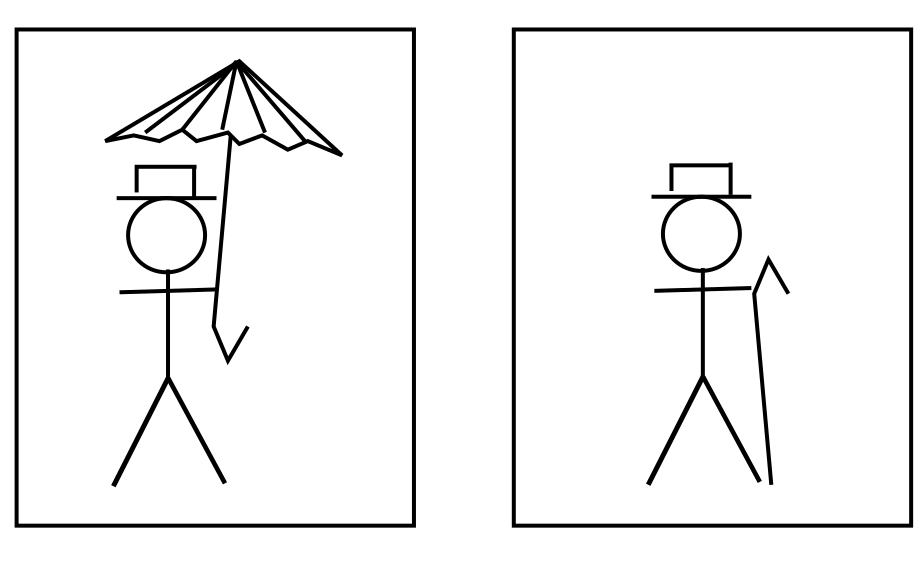
\includegraphics[width=0.8\textwidth]{files/raisonneur/reconnaissance_de_formes_0} 
\end{center}
\caption{Exemple d'environnements.}
\label{img_reco_forme_0}
\end{figure}

\begin{figure}[H] 
\begin{center}
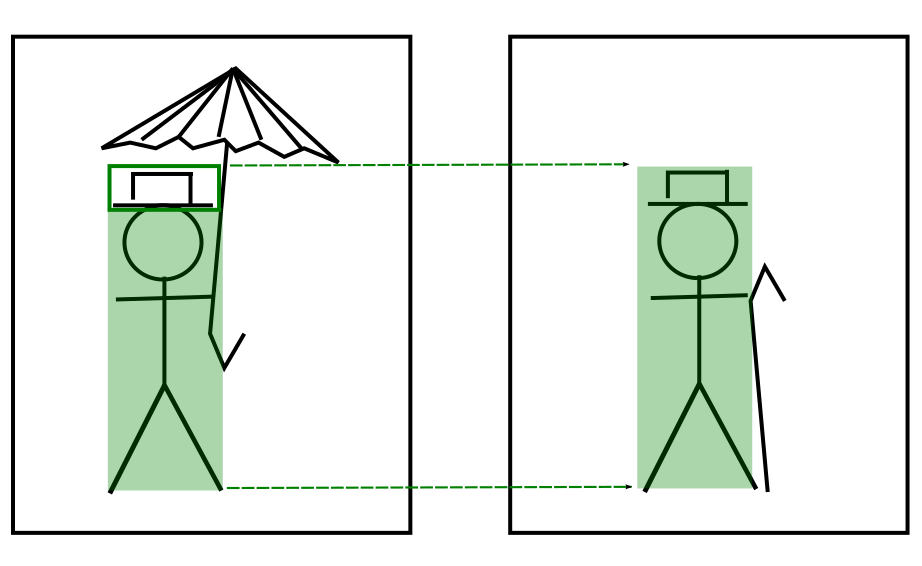
\includegraphics[width=0.8\textwidth]{files/raisonneur/reconnaissance_de_formes_injection} 
\end{center}
\caption{Exemple d'injection (basé sur la figure~\ref{img_reco_forme_0}).}
\label{img_reco_forme_injection}
\end{figure}

\subsubsection{Application aux jeux de plateau}
\label{subsection_introspection_jeux}


La figure~\ref{img_cbs_reco0} représente, de façon graphique, le type d'environnement avec lequel doit travailler le moteur d'introspection.

\begin{figure}[H] 
\begin{center}
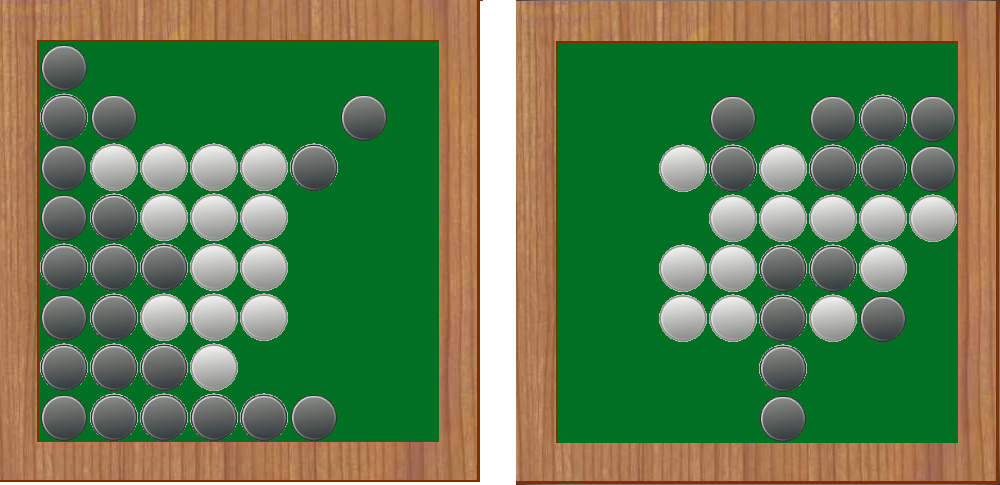
\includegraphics[width=0.7\textwidth]{files/raisonneur/cbs_reco0} 
\end{center}
\caption{Représentation graphique de l'environnement.}
\label{img_cbs_reco0}
\end{figure}

Dans un premier temps, le moteur d'introspection va rechercher en mémoire deux plateaux ayant une même annotation et présentant des formes connues identiques (cf. figure~\ref{img_cbs_reco1}). Selon notre restriction aux jeux de plateaux, l'annotation peut être \og perdant \fg{} ou \og gagnant \fg{}.

\begin{figure}[H] 
\begin{center}
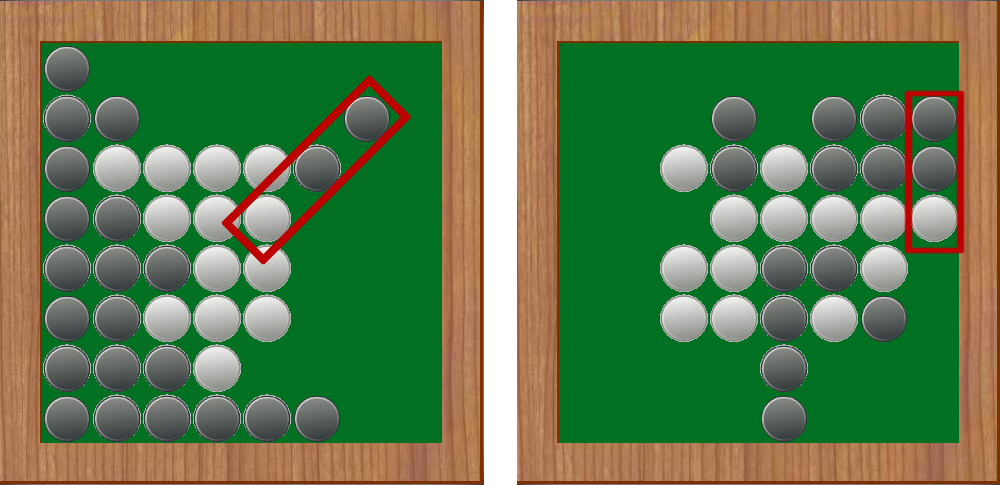
\includegraphics[width=0.7\textwidth]{files/raisonneur/cbs_reco1} 
\end{center}
\caption{Deux plateaux ayant des formes connues en commun.} 
\label{img_cbs_reco1}
\end{figure}

Le module essaye ensuite d'étendre cette forme à partir d'un des plateaux tout en vérifiant qu'elle reste présente dans l'autre plateau, comme illustré dans la figure~\ref{img_cbs_reco_forme_injection}.

\begin{figure}[H] 
\begin{center}
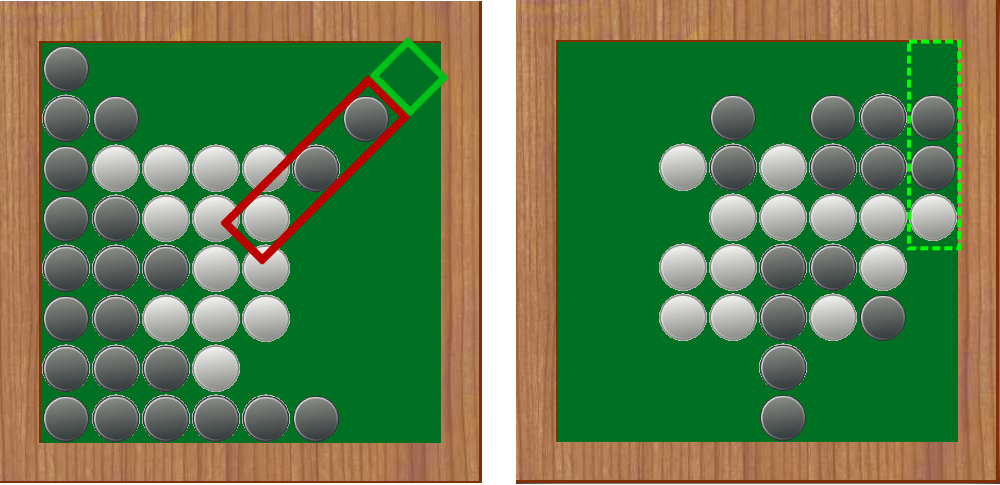
\includegraphics[width=0.7\textwidth]{files/raisonneur/cbs_reco3} 
\end{center}
\caption{Illustration de l'injection sur des plateaux.} 
\label{img_cbs_reco_forme_injection}
\end{figure}


\subsection{Valuation des formes}
\subsubsection{Cadre Général}

Pour chaque environnement annoté, le module de raisonnement effectue une mise à jour des probabilités d'apparition d'une annotation en fonction d'une forme.

\[ P(Annotation|Forme) = \frac{P(Forme|Annotation) \times P(Annotation)}{P(Forme)} \]

\paragraph{Exemple de la figure~\ref{img_annotations}}
Imaginons que nous souhaitons entraîner \cogito{} à identifier des formes géométriques basiques : \emph{rond}, \emph{carré}, \emph{croix} et \emph{triangle}. Admettons que notre IA soit capable de reconnaître dans son environnement les formes correspondantes mais qu'elle ne sache pas les associer aux annotations correspondantes.

\begin{figure}[H] 
\centering
    
\includegraphics[width=0.5\textwidth]{files/raisonneur/annotations} 
\caption{Association formes-annotations} 
\label{img_annotations}
\end{figure}

Partant de cet état initial, l'IA doit apprendre de ses expériences. Pour ce faire elle doit mettre à jour les probabilités qu'une annotation soit rattachée à un environnement pour chaque nouvel environnement rencontré. La figure~\ref{img_annotations_1} met en évidence les probabilités calculées suite à la rencontre d'un environnement présentant la forme \emph{rond}.

\begin{figure}[H] 
\centering
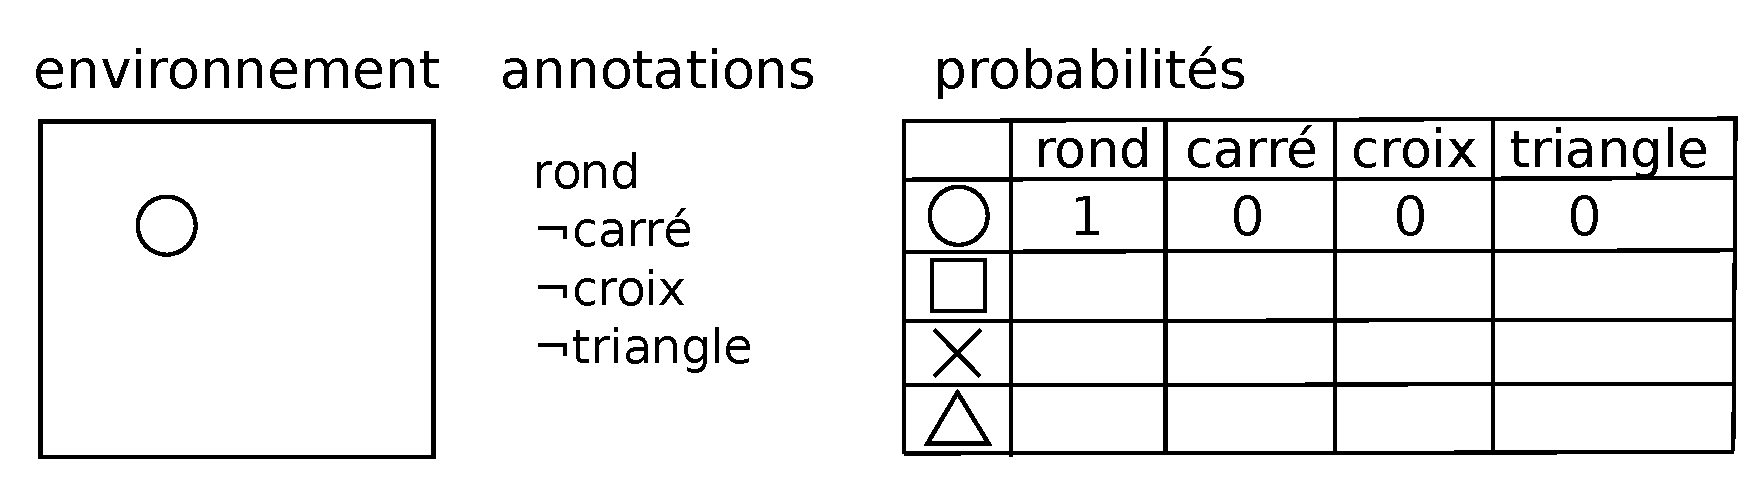
\includegraphics[width=\textwidth]{files/raisonneur/annotations_1} 
\caption{Association formes-annotations basique à l'étape 1} 
\label{img_annotations_1}
\end{figure}

Le calcul des probabilités s'effectue de la même manière pour un environnement qui présente un ensemble de formes, comme illustré sur la figure~\ref{img_annotations_2}. Il existe alors une ambiguïté car le système ne peut pas savoir quelle forme est responsable de quelle annotation.  

\begin{figure}[H] 
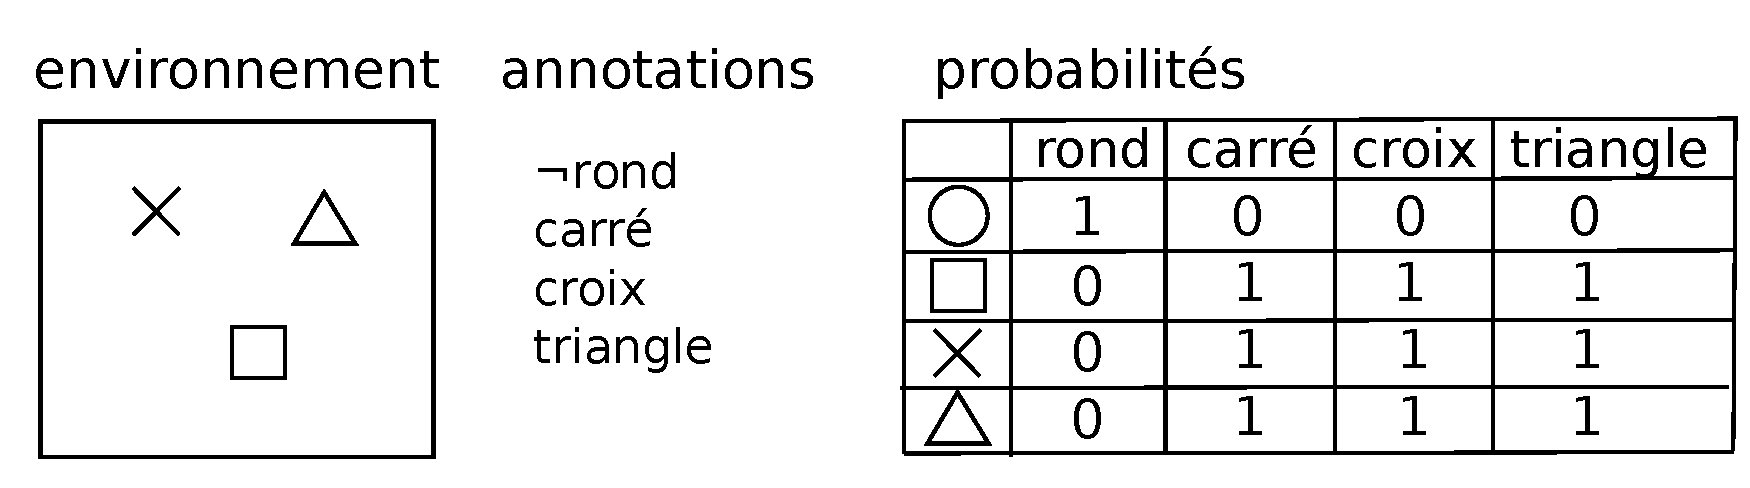
\includegraphics[width=\textwidth]{files/raisonneur/annotations_2} 
\caption{Association formes-annotations multiple à l'étape 2} 
\label{img_annotations_2}
\end{figure}

Cependant, cette ambiguïté est levée par l'expérience qui confrontera le système avec des ensembles variés de formes. Par conséquent, seul l'annotation correcte pour chaque forme conserve une probabilité certaine comme il est possible de l'observer sur les figures \ref{img_annotations_3}, \ref{img_annotations_4} et \ref{img_annotations_5} illustrant l'évolution du système. 

\begin{figure}[H] 
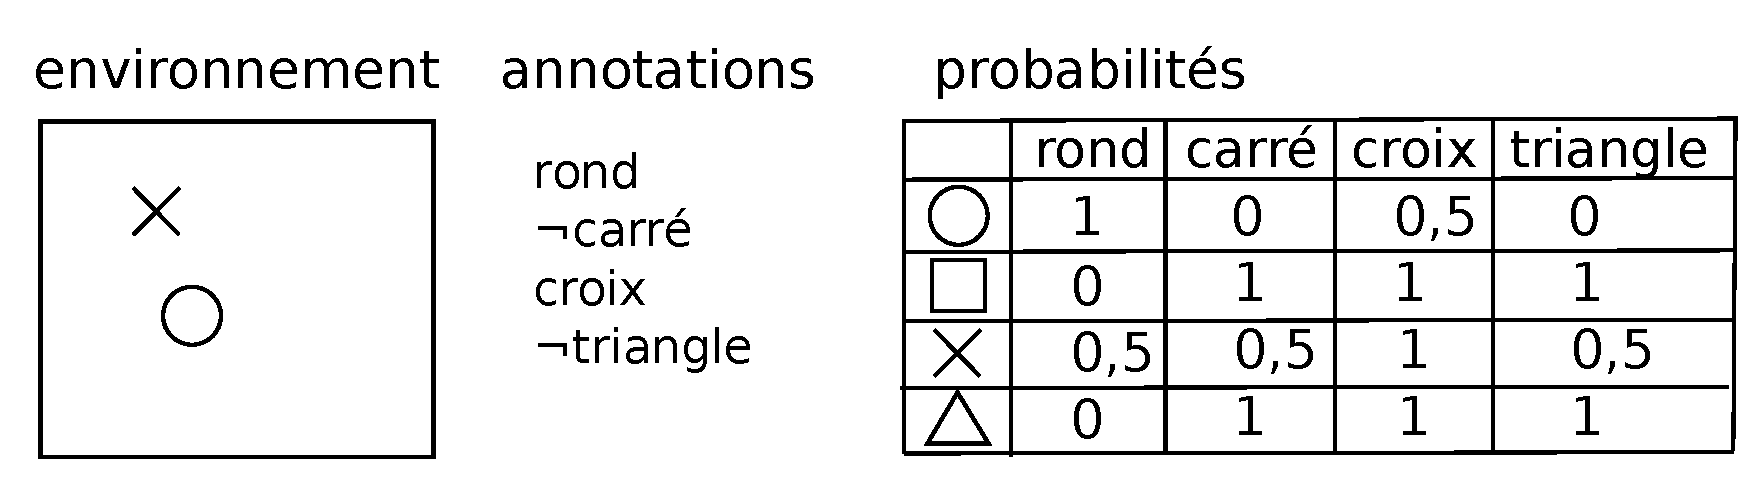
\includegraphics[width=\textwidth]{files/raisonneur/annotations_3} 
\caption{Association formes-annotations à l'étape 3} 
\label{img_annotations_3}
\end{figure}

\begin{figure}[H] 
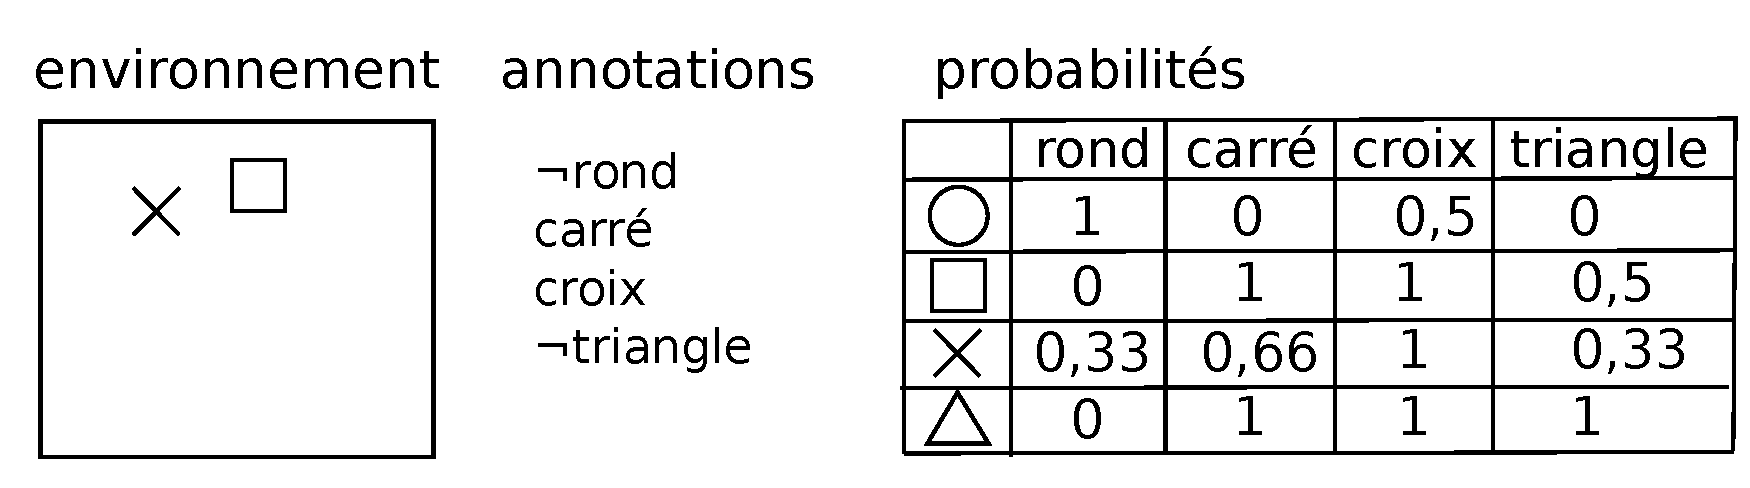
\includegraphics[width=\textwidth]{files/raisonneur/annotations_4} 
\caption{Association formes-annotations à l'étape 4} 
\label{img_annotations_4}
\end{figure}

\begin{figure}[H] 
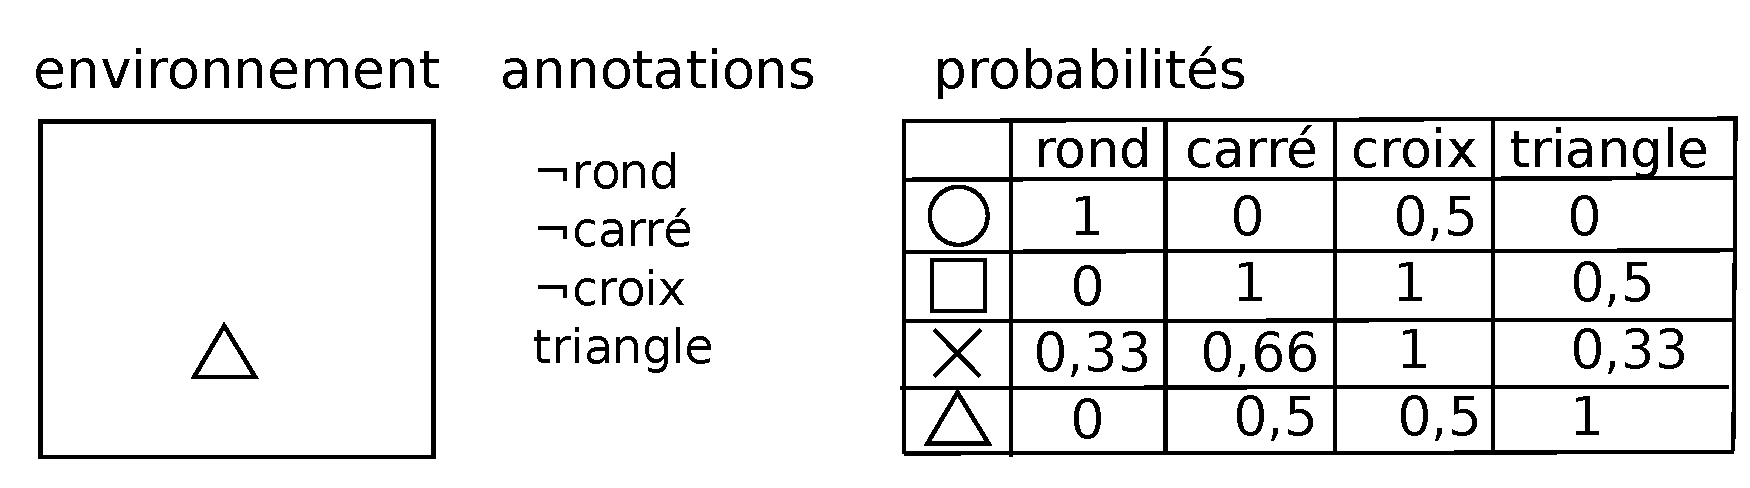
\includegraphics[width=\textwidth]{files/raisonneur/annotations_5} 
\caption{Association formes-annotations à l'étape 5} 
\label{img_annotations_5}
\end{figure}

Il est important de noter que la certitude, représentée par une probabilité égale à $1$, ne peut être garanti que si les annotations fournies au système lors de sa période d'apprentissage sont exemptes d'erreurs. Cependant, une erreur d'annotations lors de l'apprentissage certes diminuerai la probabilité associé à l'annotation correct mais pour vu que le jeux d'apprentissage soit assez grands, celle-ci resterai la plus probable.

\subsubsection{Application aux jeux de plateau}

Dans le cadre des jeux de plateau deux annotations sont fournies :
\begin{itemize}
\item \emph{victoire},
\item \emph{défaite}.
\end{itemize}
Il est évident, mais nécessaire, de préciser que :
\begin{itemize}
\item \emph{victoire} $\rightarrow{}\neg{}$ \emph{défaite}
\item \emph{défaite} $\rightarrow{}\neg{}$ \emph{victoire}
\end{itemize}

Ces annotations doivent être fournies directement par l'environnement sans intervention humaine, nous sommes donc sûr de l'apprentissage par renforcement.



\subsection{Moteur de choix}


\subsubsection{Cadre Général}

Ce module intervient après la phase d'analyse qui lui fourni, par l'intermédiaire de la mémoire, l'environnement courant et un ensemble de formes reconnues. Le \og moteur de choix \fg{} se sert alors de la probabilité d'apparition des annotations associées aux formes reconnues afin d'annoter l'environnement courant.

\subsubsection{Application aux jeux de plateau}

Dans le cadre des jeux de plateau, le moteur de choix reçoit en entrée un ensemble de plateaux avec chacun un ensemble de formes reconnues. Chaque plateau correspond au plateau résultant d'un coup possible. On peut donc dire que le moteur de choix doit choisir entre les différents \og futurs possibles \fg{}. Afin d'évaluer la probabilité de gain d'un plateau, celui-ci fera la moyenne des probabilité de gain des différentes forme reconnues sur ce plateau. Il choisi finalement l'environnement qui maximise la probabilité de gain.

\begin{figure}[H] 
  \begin{center}
		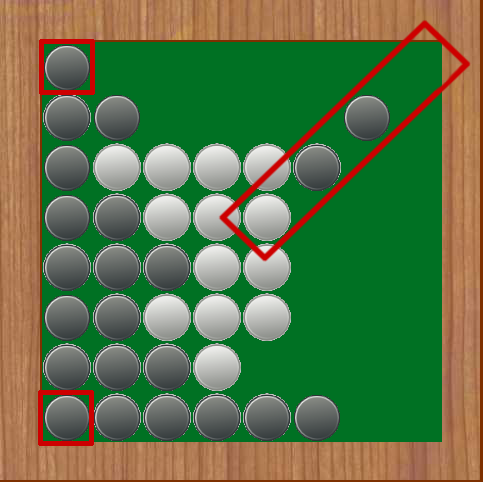
\includegraphics[width=0.3\textwidth]{files/raisonneur/moteur_de_choix} 
	\end{center}
\caption{Représentation graphique de l'environnement} 
\label{img_env}
\end{figure}



